% flashcards-title: Part-whole diagram with two known parts and an unknown whole
% flashcards-desc: Two upper boxes labeled part hold the numerals 6 and 3. Lines connect both to a wider lower box labeled whole, which holds a question mark.
\documentclass[tikz]{standalone}
\usetikzlibrary{arrows.meta,patterns}

\definecolor{qraNavy}{HTML}{17324D}
\definecolor{qraBlue}{HTML}{2B6CB0}
\definecolor{qraGold}{HTML}{B7791F}
\definecolor{qraPale}{HTML}{EAF2F8}
\definecolor{qraGray}{HTML}{5C6773}

\tikzset{
  qra axis/.style={draw=qraNavy, line width=1.2pt},
  qra tick/.style={draw=qraNavy, line width=1pt},
  qra guide/.style={draw=qraGray, densely dashed, line width=0.8pt},
  qra counter/.style={circle, draw=qraNavy, fill=qraPale, line width=0.9pt, minimum size=7mm, inner sep=0pt},
  qra label/.style={font=\sffamily\bfseries, text=qraNavy},
  qra small label/.style={font=\sffamily, text=qraNavy},
}

\begin{document}
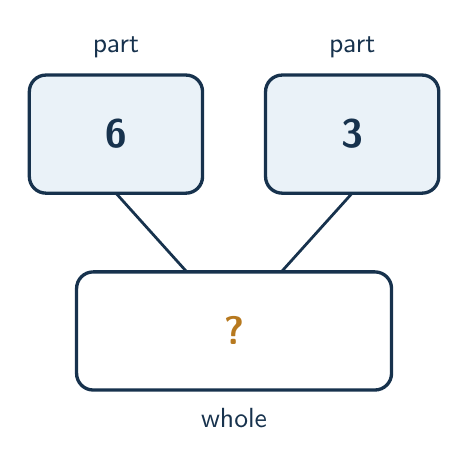
\begin{tikzpicture}
  % Part boxes
  \draw[qra axis, fill=qraPale, rounded corners=6pt] (0,0) rectangle (2.2,1.5);
  \node[qra label, font=\sffamily\bfseries\Large] at (1.1,0.75) {6};
  \node[qra small label] at (1.1,1.85) {part};

  \draw[qra axis, fill=qraPale, rounded corners=6pt] (3.0,0) rectangle (5.2,1.5);
  \node[qra label, font=\sffamily\bfseries\Large] at (4.1,0.75) {3};
  \node[qra small label] at (4.1,1.85) {part};

  % Whole box
  \draw[qra axis, fill=white, rounded corners=6pt] (0.6,-2.5) rectangle (4.6,-1.0);
  \node[qra label, font=\sffamily\bfseries\Large, text=qraGold] at (2.6,-1.75) {?};
  \node[qra small label] at (2.6,-2.85) {whole};

  % Connectors from each part to the whole
  \draw[qra tick] (1.1,0) -- (2.0,-1.0);
  \draw[qra tick] (4.1,0) -- (3.2,-1.0);
\end{tikzpicture}
\end{document}
